\documentclass[inlineanswers]{exam2024}
%\documentclass[noanswers]{exam2023}

\usepackage[utf8]{inputenc}
\usepackage{hyperref,booktabs}
\usepackage{amsmath, amsfonts,sansmath,bm, amsthm,MnSymbol}
\usepackage{graphicx} 
\usepackage{float} 

\begin{document}

\paper{Graph Representation Learning}
\begin{abstract}
\noindent
Oversmoothing and over-squashing are two types of failures of information propagation in graph neural networks (GNNs): the first destroys signal essentially by too much mixing at depth, the latter by too little signal surviving a topological bottleneck. Two methods target them separately - residual (skip) connections for oversmoothing (as tested in one of our practicals) and graph rewiring for over-squashing. This miniproject studies whether these remedies complement each other or whether fixing one failure mode worsens the other. Using two controlled synthetic datasets (a stochastic block model for oversmoothing, a barbell signal-propagation task for over-squashing) and a $2\times2$ design over \{plain, skip\}$\times$\{original, rewired\}, evaluated across five seeds, we find a (fairly interesting but in the end not surprising) trade-off: curvature-based rewiring - as anticipated - fixes over-squashing but worsens oversmoothing, while skip connections mitigate oversmoothing + moderate over-squashing but fail on longer bottlenecks. Only the combination is robust on both axes. The mechanism is checked with Jacobian-sensitivity and Ollivier-Ricci curvature metrics.
\end{abstract}

\begin{center}
\small Code: \url{https://anonymous.4open.science/r/Graph_Representation_Learning_Miniproject-832F} 
\end{center}

\section{Introduction}
\label{sec:intro}

Message-passing GNNs propagate information by essentially repeatedly aggregating neighbour features. This single mechanism underlies two well-documented and opposite pathologies of information propagation:

\textbf{Oversmoothing}: as the depth grows, repeated averaging drives all node representations toward a common vector, so deeper networks become less discriminative
\cite{li2018deeper,oono2020,rusch2023survey}. 

\textbf{Over-squashing}: when a task requires information to travel through a structural bottleneck, an "exponentially growing receptive field" is compressed into a fixed-width vector and long-range signal is lost \cite{alon2021,topping2022,digiovanni2023}.

The two remedies presented in the lecture are usually studied in isolation. \emph{Skip connections} \cite{xu2018jk} add a node's previous-layer representation back at each layer, counteracting oversmoothing. \emph{Graph rewiring}
\cite{topping2022} alters the input topology to relieve bottlenecks; Stochastic Discrete Ricci Flow (SDRF) adds edges at the most negatively curved (bottleneck) locations. Because the two pathologies could be called opposites, a natural and - to my
knowledge - underexamined question is whether the two fixes interfere with each other.

\paragraph{Research question.}
\emph{Do skip connections and graph rewiring complement each other in addressing oversmoothing and over-squashing , or does fixing the one worsen the other?} This matters because by mitigating one of the issues, researchers/practitioners could in theory worsen the other one without noticing right away.

\section{Methods}
\label{sec:methods}

\paragraph{Approach and goals.}
Each pathology is isolated in a synthetic graph where its severity is controllable via its parameters, and looked into via a $2\times2$ grid: model
$\in\{\text{GCN},\text{SkipGCN}\}$ and topology $\in\{\text{original},\text{rewired}\}$,
resulting in four cases: \textsc{GCN}, \textsc{SkipGCN}, \textsc{GCN+Rewire}, \textsc{Skip+Rewire}.
The goal is to read off which mitigation technique helps or hurts which pathology.

\paragraph{Models.}
Both models stack K basic \texttt{GCNConv} layers (hidden width $64$, ReLU, dropout
$0.3$). \textsc{SkipGCN} uses the in Practical-3 introduced residual update
$\bm{H}^{(t)}=\mathrm{ReLU}\big(\mathrm{GCNConv}(\bm{H}^{(t-1)})\big)+
\mathrm{proj}(\bm{H}^{(t-1)})$, where $\mathrm{proj}$ is a linear map when widths differ and identity otherwise.

\paragraph{Graph A: oversmoothing (SBM).}
A stochastic block model with $4$ communities of $50$ nodes ($p_{\text{intra}}{=}0.7$,
$p_{\text{inter}}{=}0.02$, $16$ random Gaussian features); node task = classify community. Dense intra-community connections make the repeated averaging collapse the node embeddings.

\paragraph{Graph B: over-squashing (barbell).}
Two $5$-cliques joined by a bridge of length $b$ (Fig.~\ref{fig:topology}). A binary signal is out at a sourcenode in the left clique; all other nodes carry only random noise. The model must predict the signal only at a target node in
the right clique, so the answer has to cross the bridge (distance $1{+}b$ hops) for it to work. Loss and accuracy are read at the target node, preventing any pooling shortcut. Sweep goes over depth $K$ and bridge length $b$ independently. $400$ graphs per setting are used, in a classic $60/20/20$ train/val/test split.

\paragraph{Rewiring.}
Here, an SDRF-inspired rewiring is used: each step targets the most negatively curved edge (Ollivier-Ricci, $\alpha{=}0$) and adds a shortcut between its low-degree neighbours. This differs from \cite{topping2022} mainly in the edge-selection rule (here: deterministic, degree-based, rather than softmax-curvature improvement approach); Hence it is ``SDRF-inspired''. Fig.~\ref{fig:topology} shows it removes the negative-curvature bridge edges and adds additional shortcuts.

\paragraph{Diagnostics \& protocol.} 
Oversmoothing is measured by MAD (mean pairwise cosine distance of embeddings) and Dirichlet energy \cite{li2018deeper,rusch2023survey}; over-squashing by the Jacobian sensitivity $\lVert\partial \bm h_v/\partial \bm x_u\rVert$ vs.\ $u$–$v$ distance \cite{topping2022,digiovanni2023}. Adam is used (SBM full-batch, lr~$0.01$; barbell mini-batched, lr~$0.005$, batch~$32$) with early stopping on a validation split. All results are mean $\pm$ std over 5 seeds; the SBM is fixed (seeds vary initialisation), the barbell is re-drawn per seed. Main assumption is that the synthetic graphs isolate each pathology and that MAD/Jacobian are valid proxies.

\begin{figure}[t]
\centering
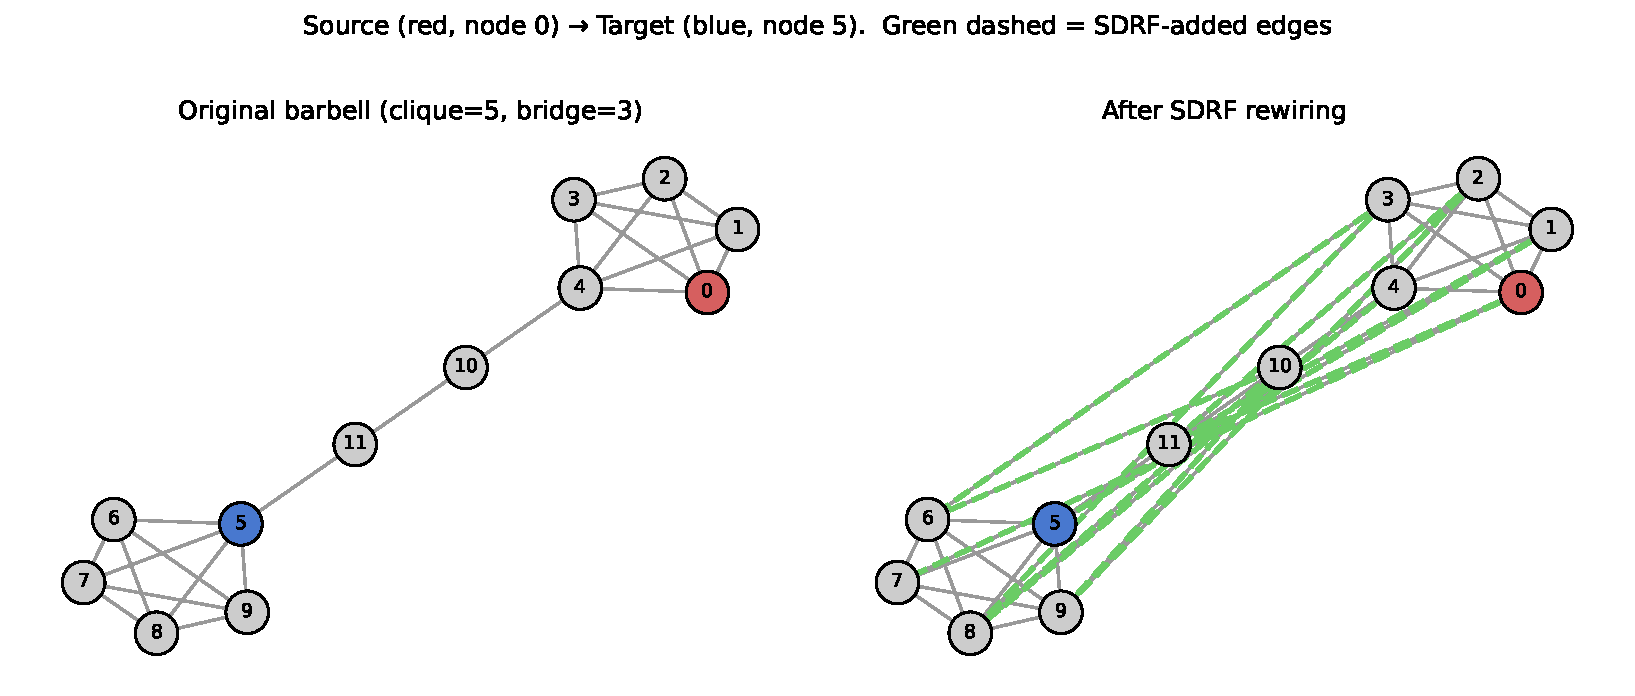
\includegraphics[width=0.86\linewidth]{barbell_topology.pdf}
\caption{Barbell task before/after SDRF-inspired rewiring. Source (red) and target (blue) are separated by a thin bridge (negative curvature); rewiring (the green dashed edges) connects the clusters directly, collapsing the diameter from $5$ to $2$.}
\label{fig:topology}
\end{figure}

\section{Results}
\label{sec:results}

\paragraph{Rewiring removes the bottleneck.}
The barbell has exactly $4/23$ negatively curved edges (== the bridge) and SDRF eliminates them, shifting the whole curvature distribution positive (App.~\ref{app:curv}). This merely confirms that the intervention does what it should before going into answering the research question.

\paragraph{Experiment A - oversmoothing (Fig.~\ref{fig:expA}).}
Plain GCN collapses with depth as expected and already tested in the practicals: accuracy $1.0\!\to\!0.19\pm.03$ at $K{=}16$ and
MAD $0.343\pm.037$ $\to 0.000\pm.000$. Skip connections substantially mitigate this (Acc $0.97\pm.03$ at $K{=}8$) but do not fully solve it:
at $K{=}16$ they are $0.86\pm.26$ - high variance, i.e.\ some initialisations still
fail (as could be seen in the practicals). 

Most importantly, \textbf{rewiring worsens oversmoothing}: \textsc{GCN+Rewire}
($0.44\pm.15$ at $K{=}8$) is below \textsc{GCN} ($0.64\pm.23$), with lower MAD, because the added edges increase connectivity and hence accelerate the neighbour-averaging that drives the collapse.


\paragraph{Experiment B - over-squashing (Fig.~\ref{fig:expB}, Table~\ref{tab:bridge} in App.~\ref{app:bridge})).}
With depth (bridge $b{=}3$, $4$ hops needed), GCN never reliably solves the task at
any $K$ (e.g.\ $0.57\pm.22$ at $K{=}8$), whereas \textsc{SkipGCN} is ''perfect'' for
$K\ge8$ ($1.000\pm.000$). Going from there, sweeping bridge length from 1 to 7 at $K{=}8$ gives the result that under the given circumstances rewiring solves over-squashing at every bridge length ($1.000\pm.000$ throughout),
while skip connections degrades slowly but surely - perfect at $b{=}3$, bimodal at $b{=}4$
($0.73\pm.23$), and essentially broken from $b\ge5$ ($0.46\pm.04$). At
$b{=}4\text{-}5$ skip alone starts becoming insufficient but rewiring still succeeds.

\paragraph{Experiment C - propagation mechanism (Fig.~\ref{fig:expC}).}
Jacobian sensitivity decays with distance for all models, but \textsc{SkipGCN}
retains $100$-$600\times$ more long-range sensitivity than \textsc{GCN} at every
distance (gap fairly robust to seed variance), explaining why it transports the signal
further\footnote{Rewired graphs have datapoints only up to distance $2$: SDRF shrank the
diameter so no longer-range pairs exist - itself direct evidence the bottleneck is
gone.}.

\paragraph{Summary.}
Table~\ref{tab:summary} consolidates the $K{=}8$ slice. One can say that the hypothesis is
supported: the two interventions are complementary but partially asymmetric, and
\textsc{GCN+Rewire} is the cell that proves the trade-off is real in these circumstances - best on the over-squashing axis, worst on the oversmoothing axis.

\begin{figure}[H]
\centering
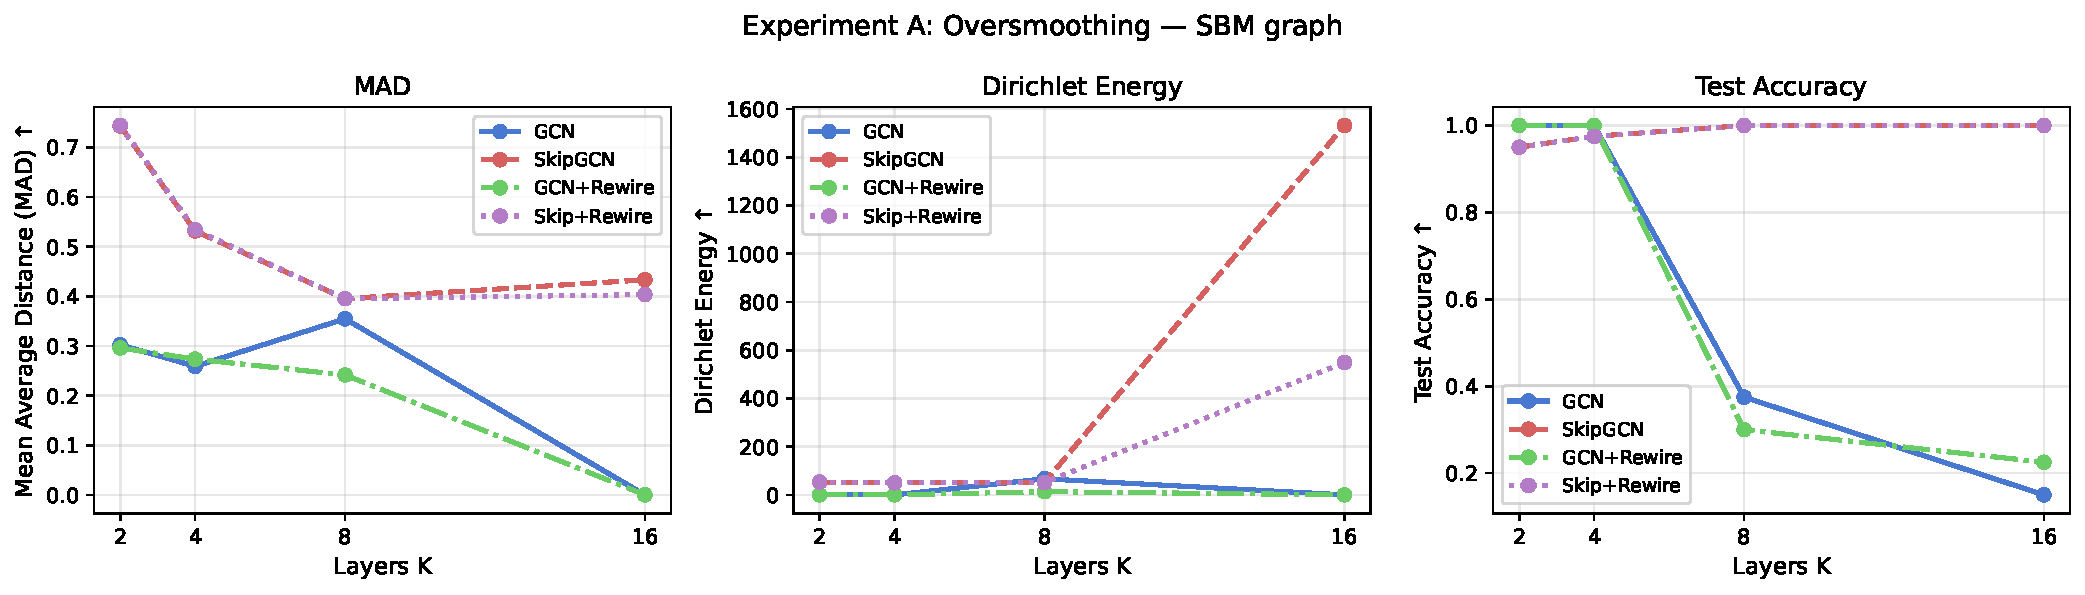
\includegraphics[width=0.98\linewidth]{exp_a_oversmoothing.pdf}
\caption{Experiment A (SBM, mean$\pm$std over 5 seeds). GCN collapses with depth
(MAD$\to0$, Acc$\to$chance); skip connections mitigate but show large variance at
$K{=}16$; rewiring lowers MAD and accuracy relative to its non-rewired counterpart.}
\label{fig:expA}
\end{figure}

\begin{figure}[H]
\centering
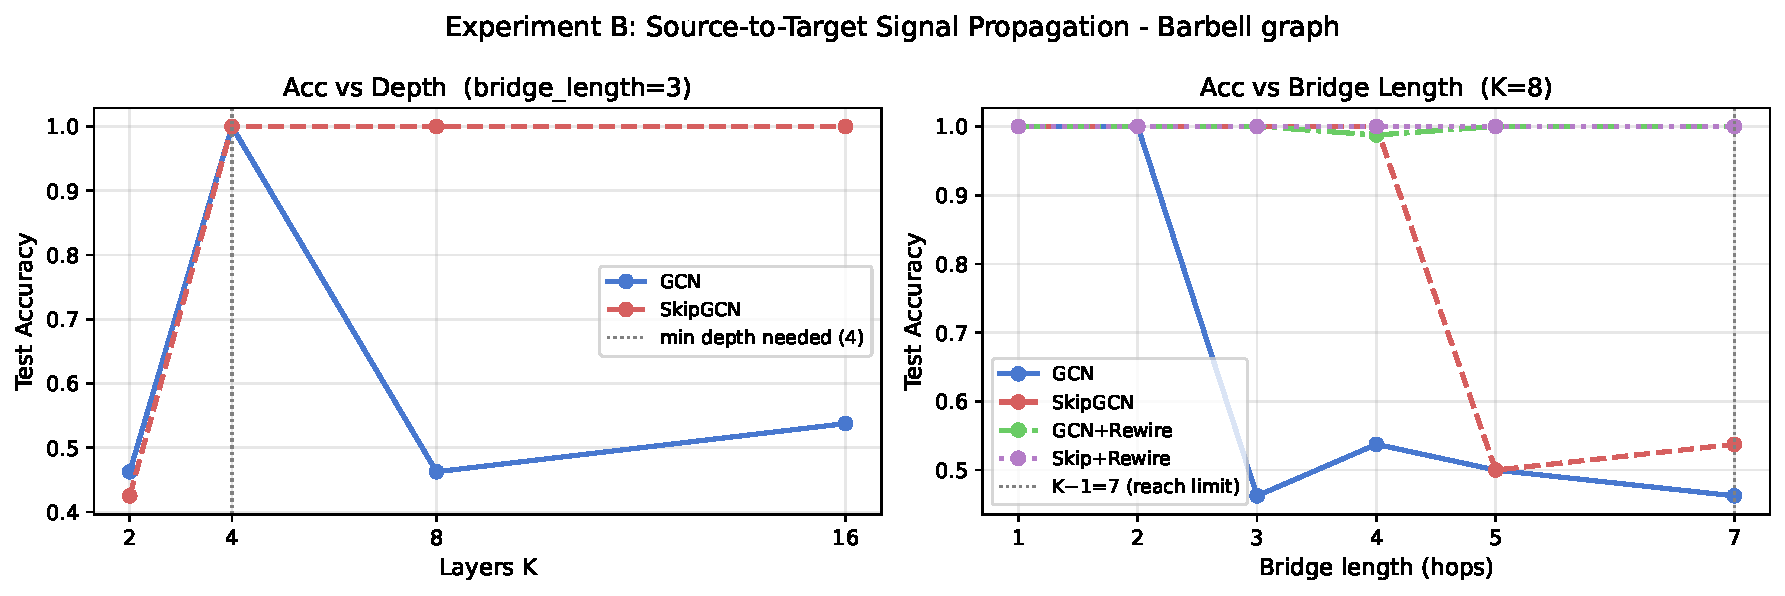
\includegraphics[width=0.98\linewidth]{exp_b_oversquashing.pdf}
\caption{Experiment B (barbell, mean$\pm$std over 5 seeds). Left: accuracy vs.\ depth
($b{=}3$). Right: accuracy vs.\ bridge length ($K{=}8$). Rewired conditions are at
$1.0$ throughout; \textsc{SkipGCN} fails for $b\ge5$.}
\label{fig:expB}
\end{figure}

\begin{figure}[H]
\centering
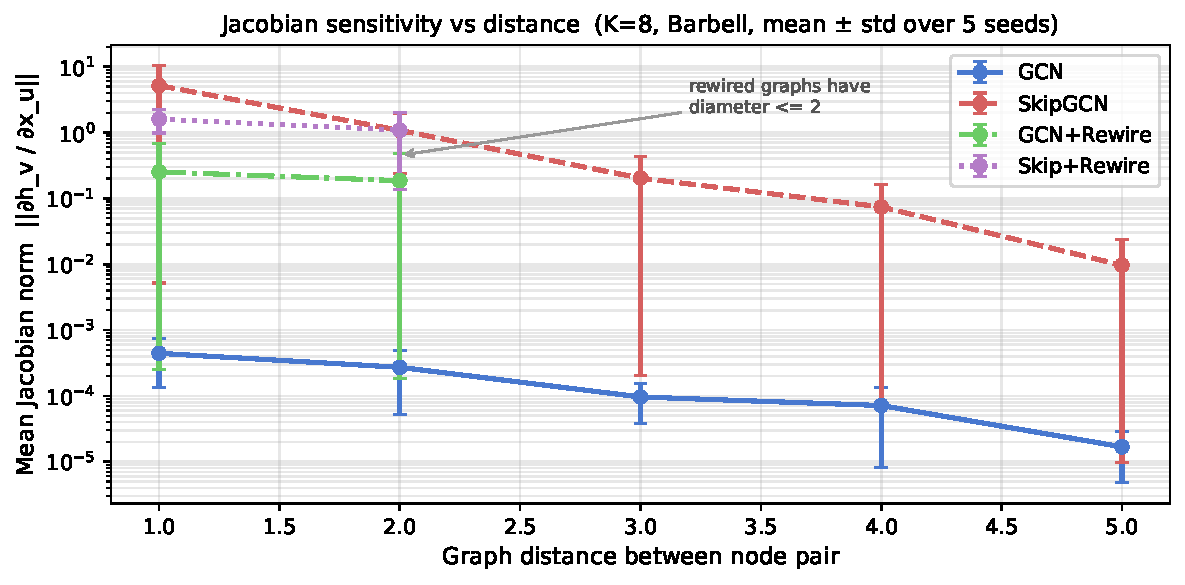
\includegraphics[width=0.7\linewidth]{exp_c_jacobian.pdf}
\caption{Experiment C: Jacobian sensitivity vs.\ distance ($K{=}8$, mean$\pm$std over
5 seeds). \textsc{SkipGCN} retains far more long-range sensitivity; SRDF rewired curves
stop at distance $2$ because the diameter shrinks.}
\label{fig:expC}
\end{figure}

\begin{table}[t]
\centering
\small
\caption{Summary at $K{=}8$ (mean$\pm$std over 5 seeds). }
\label{tab:summary}
\begin{tabular}{lccc}
\toprule
Model & MAD (SBM) & Acc (SBM) & Acc (Barbell $b{=}3$)\\
\midrule
\textsc{GCN}          & .329$\pm$.047 & .640$\pm$.227 & .565$\pm$.218 \\
\textsc{SkipGCN}      & .381$\pm$.040 & .965$\pm$.034 & \textbf{1.000$\pm$.000} \\
\textsc{GCN+Rewire}   & .290$\pm$.056 & .440$\pm$.147 & \textbf{1.000$\pm$.000} \\
\textsc{Skip+Rewire}  & .379$\pm$.028 & .970$\pm$.037 & \textbf{1.000$\pm$.000} \\
\bottomrule
\end{tabular}
\end{table}

\section{Discussion}
\label{sec:discussion}

\paragraph{Critical perspective.}
There are a few things that can and should be improved upon in the future as this ''miniproject'' was done in a limited scope and time:

\begin{part}
    Rewiring ``wins'' partly by changing the task: SDRF collapses the source-target distance to $1$-$2$ hops, so at $K{=}8$ the problem becomes trivial - the perfect $1.000\pm.000$ reflects an easier graph, not a model that squashes less. 
    \item The barbell metric is bimodal (the runs either solve it, $\approx1.0$, or sit at chance, $\approx0.5$); a mean of $0.73$ means roughly ``$3/5$ seeds solved it,'' not a typical $73\%$. 
    \item Skip connections are a \emph{mitigation, not a cure}: at $K{=}16$ ($.86\pm.26$) and $b{=}4$ ($.73\pm.23$) they are unreliable. A note that was already taken in the practicals though.
    \item The Jacobian's absolute scale is unstable across seeds (e.g.\ SkipGCN $5.2\pm5.2$ at distance $1$); At least the decay and the gaps can be seen as useful.
    \item Last but not least: The datasets are small and synthetic (by design); they are supposed to isolate the mechanisms but obviously do not provide results on real and more complex graphs.
\end{part}

\section{Conclusions and Outlook}
\label{sec:conclusion}

In this controlled $2\times2$ study we see that skip connections and curvature-based
rewiring are complementary but asymmetric: rewiring seems to fix the
over-squashing but worsens oversmoothing; skip connections mitigate oversmoothing
and moderate over-squashing but fail on longer bottlenecks, and only their
combination is robust on both. Practically, ``stacking fixes'' seem to be justified here, but each fix has a cost on the opposite side.

\paragraph{Outlook.}
To study this in more detail following points are to be considered in the future: 

(i) Test on real(life) long-range benchmarks to see whether the trade-off persists beyond synthetic graphs;

(ii) Fully implemented SDRF (softmax-sampled by curvature gain) and alternative rewiring strategies to separate the current ``shortening the path'' from ``actually changing the curvature'';

(iii) a graph dataset where rewiring cannot trivially shorten the source-target
distance; essentially to test rewiring's benefit when it does not change the task difficulty.

\begin{thebibliography}{99}
\small
\bibitem{li2018deeper} Q.~Li, Z.~Han, X.-M.~Wu. Deeper insights into graph convolutional networks for semi-supervised learning. \emph{AAAI}, 2018.

\bibitem{oono2020} K.~Oono, T.~Suzuki. Graph neural networks exponentially lose
expressive power for node classification. \emph{ICLR}, 2020.

\bibitem{rusch2023survey} T.~K.~Rusch, M.~M.~Bronstein, S.~Mishra. A survey on
oversmoothing in graph neural networks. \emph{arXiv:2303.10993}, 2023.

\bibitem{alon2021} U.~Alon, E.~Yahav. On the bottleneck of graph neural networks and
its practical implications. \emph{ICLR}, 2021.

\bibitem{topping2022} J.~Topping, F.~Di~Giovanni, B.~Chamberlain, X.~Dong,
M.~Bronstein. Understanding over-squashing and bottlenecks on graphs via curvature.
\emph{ICLR}, 2022.

\bibitem{digiovanni2023} F.~Di~Giovanni, L.~Giusti, F.~Barbero, et al. On
over-squashing in message passing neural networks: the impact of width, depth, and
topology. \emph{ICML}, 2023.

\bibitem{xu2018jk} K.~Xu, C.~Li, Y.~Tian, et al. Representation learning on graphs
with jumping knowledge networks. \emph{ICML}, 2018.

\bibitem{kipf2017} T.~N.~Kipf, M.~Welling. Semi-supervised classification with graph
convolutional networks. \emph{ICLR}, 2017.

\end{thebibliography}

\appendix
\section{Curvature distribution}
\label{app:curv}
\begin{figure}[h]
\centering
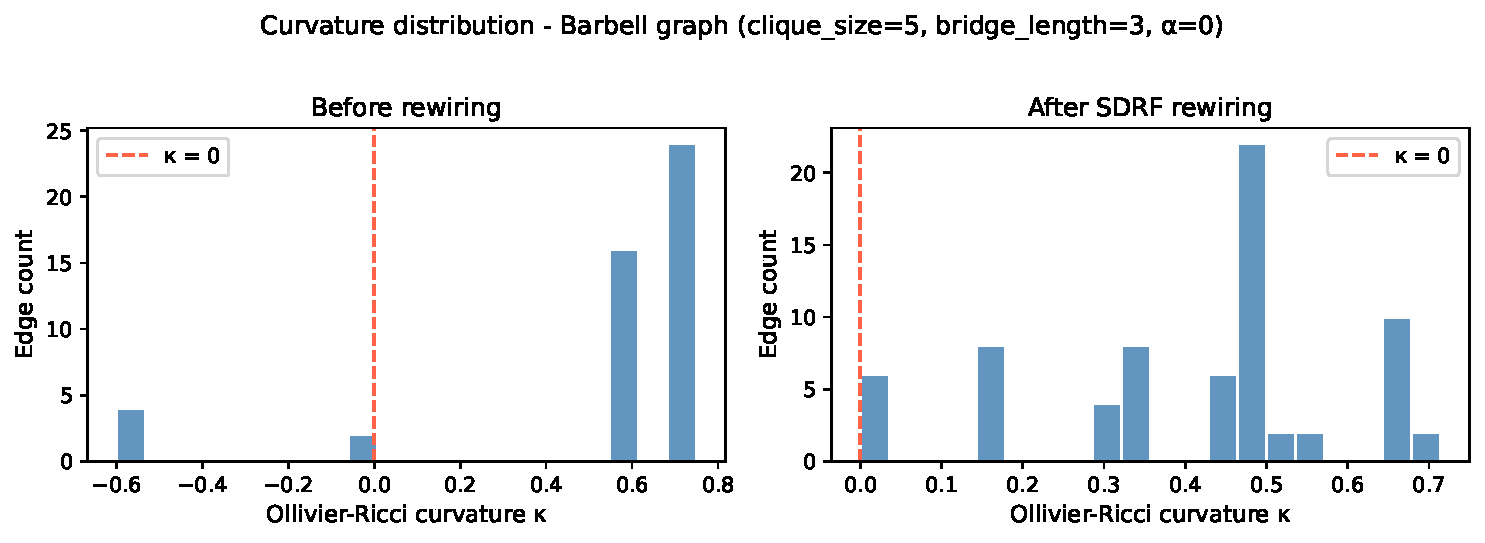
\includegraphics[width=0.86\linewidth]{curvature_distributions.pdf}
\caption{Ollivier-Ricci curvature of the barbell before/after rewiring. The negative
(bottleneck) edges are removed and the distribution shifts positive.}
\end{figure}

\section{Oversquashing over bridge-length}
\label{app:bridge}
\begin{table}[t]
\centering
\small
\caption{Over-squashing: target-node accuracy vs.\ bridge length ($K{=}8$,
mean$\pm$std over 5 seeds). Rewiring is invariant to bridge length; skip connections
break at $b\ge5$.}
\label{tab:bridge}
\begin{tabular}{lcccccc}
\toprule
$b$ (hops) & 1 & 2 & 3 & 4 & 5 & 7 \\
\midrule
\textsc{GCN}          & 1.00 & .90$\pm$.20 & .57$\pm$.22 & .50$\pm$.04 & .50$\pm$.02 & .49$\pm$.04 \\
\textsc{SkipGCN}      & 1.00 & 1.00 & 1.00 & .73$\pm$.23 & .46$\pm$.04 & .51$\pm$.04 \\
\textsc{GCN+Rewire}   & 1.00 & 1.00 & 1.00 & 1.00 & 1.00 & 1.00 \\
\textsc{Skip+Rewire}  & 1.00 & 1.00 & 1.00 & 1.00 & 1.00 & 1.00 \\
\bottomrule
\end{tabular}
\end{table}

\end{document}